\documentclass[review]{elsarticle}


\usepackage{lineno,hyperref}
\newtheorem{definition}{Definition}
\usepackage{amssymb,amsmath,array}
\usepackage{xcolor}% provides \colorlet
\usepackage{fixme}
\fxsetup{
    status=draft,
    author=,
    layout=inline,
    theme=color
}

\definecolor{fxnote}{rgb}{0.8000,0.0000,0.0000}
% define the background colour:
\colorlet{fxnotebg}{yellow}

% refedine the layout macro:
\makeatletter
\renewcommand*\FXLayoutInline[3]{%
  \@fxdocolon {#3}{%
    \@fxuseface {inline}%
    \colorbox{fx#1bg}{\color {fx#1}\ignorespaces #3\@fxcolon #2}}}
\makeatother

\modulolinenumbers[5]

\journal{Journal of \LaTeX\ Templates}

\newcommand{\IR}{\rm I\!R}

%%%%%%%%%%%%%%%%%%%%%%%
%% Elsevier bibliography styles
%%%%%%%%%%%%%%%%%%%%%%%
%% To change the style, put a % in front of the second line of the current style and
%% remove the % from the second line of the style you would like to use.
%%%%%%%%%%%%%%%%%%%%%%%

%% Numbered
%\bibliographystyle{model1-num-names}

%% Numbered without titles
%\bibliographystyle{model1a-num-names}

%% Harvard
%\bibliographystyle{model2-names.bst}\biboptions{authoryear}

%% Vancouver numbered
%\usepackage{numcompress}\bibliographystyle{model3-num-names}

%% Vancouver name/year
%\usepackage{numcompress}\bibliographystyle{model4-names}\biboptions{authoryear}

%% APA style
%\bibliographystyle{model5-names}\biboptions{authoryear}

%% AMA style
%\usepackage{numcompress}\bibliographystyle{model6-num-names}

%% `Elsevier LaTeX' style
\bibliographystyle{elsarticle-num}
%%%%%%%%%%%%%%%%%%%%%%%

\begin{document}

\begin{frontmatter}

\title{The Conjunctive Disjunctive Graph Node Kernel for Disease Gene Prioritization}
%\tnotetext[mytitlenote]{Fully documented templates are available in the elsarticle package on \href{http://www.ctan.org/tex-archive/macros/latex/contrib/elsarticle}{CTAN}.}

%% Group authors per affiliation:
\author{Dinh Tran Van}
\author{Alessandro Sperduti}
\address{Department of Mathematics, Padova University, Trieste, 63, 35121 Padova, Italy}
\author{Fabrizio Costa}
\address{Department of Computer Science, University of Exeter Exeter EX4 4QF, UK}
%\fntext[myfootnote]{Since 1880.}

%% or include affiliations in footnotes:
%\author[mymainaddress,mysecondaryaddress]{Elsevier Inc}
%\ead[url]{www.elsevier.com}

%\author[mysecondaryaddress]{Global Customer Service\corref{mycorrespondingauthor}}
%\cortext[mycorrespondingauthor]{Corresponding author}
%\ead{support@elsevier.com}

%\address[mymainaddress]{1600 John F Kennedy Boulevard, Philadelphia}
%\address[mysecondaryaddress]{360 Park Avenue South, New York}

\begin{abstract}
Biological relations encoded in data sources are naturally represented in the form of graphs. As a consequence, a high number of graph-based biological learning systems have been proposed and shown promissing results. In graph-based learning systems, one of the key points which determines their performance is the denifition of graph node similarity measure. Node similarities are normally measured by graph node kernels. However, most available graph node kernels do not show high discriminative capacity since they share two common limitations. First they are based on the diffusion phenomenon which does not effectively exploit the nodes' configuration. Second they are not able to proceed the auxiliary information associated to graph nodes.

In this paper, we propose an efficient graph node kernel that not only effectively exploits nodes' context, but also process with additional information which available on the graph nodes. Empirical evaluation on disease gene prioritization show that our proposed graph node kernel shows the state of the art concerning graph node kernels.

%Gene-disease associations are inferred on the basis of similarities between the proteins encoded by genes. Biological relationships used to define similarities range from interacting proteins, proteins that participate in pathways and protein expression profiles. Though graph kernel methods have become a prominent approach for association prediction, most solutions are based on a notion of information diffusion that does not capture the specificity of different network parts. Here we propose a graph kernel method that explicitly models the configuration of each gene's context. An empirical evaluation on several biological databases shows that our proposal achieves state-of-the-art results.
\end{abstract}

\begin{keyword}
Graph node kernels, graph decomposition, disease gene prioritization
\end{keyword}
\end{frontmatter}

\linenumbers
\section{Introduction}
The release of advanced technologies is one of the main reasons for the
revolution in various scientific research fields. In Biological and Medical
domain, modern technologies are making it not only easier but also more
economical than ever to undertake experiments and creating applications.
As a consequence, a vast amount of biological data in terms of volume
and type is generated through scientific experiments, published literature,
high-throughput experiment technology, and computational analysis. This
huge quantity of data are saved as biological datasets and made discoverable
through web browsers, application programming interfaces, scalable search
technology and extensive cross-referencing between databases. Biological
databases normally contain information about gene function, structure, lo-
calization, clinical effects of mutations and similarities of biological sequences and structures.

In Biomedical, disease-gene association recovery is a major goal in molecular  that has received much attention from many researchers. Despite that fact that a big progress has been made in the last decades, a number of genes known to be related to a genetic disease is normally limited. In order to find out the complement set of the known disease gene set, one way is to search for whole genome or specific regions that often contain a large number of suspected genes (candidate genes). This is obvious not a good idea as it is expensive not only in term of time consuming but also from financial aspect. For this reason, a considerable number of gene prioritization methods have been proposed. Predictive systems for gene-disease associations are often based on a notion of similarity between genes. A common strategy is to encode relations between genes as a network and to use graph based techniques to make useful inferences \cite{mordelet2011prodige}, \cite{chen2014disease}, \cite{valentini2014extensive}.

One of the key points that determines the performance of graph-based biological learning systems in general and graph-based disease gene prioritization systems in particular is the definition of node similarity measure. The node similarity is often measured by graph node kernels \cite{kondor2002diffusion}, \cite{chen2014disease}, \cite{fouss2006experimental}, \cite{chebotarev2006matrix}. However, the state of the art graph node kernels used to measure node similarity, are based on the notion of information diffusion. These graph node kernels often show relatively low discriminative capacity, especially in cases of working with sparse graphs, graphs have high numbers of missing links, since they share following limitations. First information is processed in an additive and independent fashion which prevents them from accurately modeling the configuration of each node's context. Second, they do not take into account information associated to nodes of graphs when they are available. These additional information normally provide a complement to graph topology. Therefore, they are potential to use to improve the expressiveness of graph node kernels. 

We propose an effective convolutional graph node kernel, named \textit{Conjunctive disjunctive node kernel} (CDNK) which is able to \textit{i}) effectively exploit the nodes' context, \textit{ii}) process with information sticked on nodes of graphs.

\section{Background}
In this section, we first introduce definitions and notations that are used to define our proposed method. We then describe the state-of-the-art concerning graph node kernels.
\subsection{Definitions and Notations}
A graph is a structure $G=(\mathbb{V},\mathbb{E}, \mathcal{L}_1, \mathcal{L}_2)$ where $\mathbb{V}$, $\mathbb{E}, \mathcal{L}_1, \mathcal{L}_2$ are the vertex (node) set, link (edge) set, discrete labeling fuction and real vector labeling function, respectively. The functions $\mathcal{L}_1, \mathcal{L}_2$ are defined as:
\begin{itemize}
\item $\mathcal{L}_1: \mathbb{V} \longmapsto \mathbb{L}$, where $\mathbb{L}$ is a set of discrete labels. $\mathcal{L}_1$ assigns a single discrete label $\ell \in \mathbb{L}$ for each ndoe $v \in \mathbb{V}$, $\mathcal{L}_1(v) = \ell$. 
\item $\mathcal{L}_2: \mathbb{V} \longmapsto \mathbb{R}^n$. $\mathcal{L}_2$ assigns a single real vector label $(v_1,v_2,\ldots,v_n) \in \mathbb{R}^n$ for each ndoe $v \in \mathbb{V}$, $\mathcal{L}_2(v) = (v_1,v_2,\ldots,v_n)$.
\end{itemize}

We define the shortest path between $u$ and $v$, notated as $\mathcal{D}(u,v)$, as the number of edges on the shortest path between them. The \textit{neighborhood} of a node $u$ with radius $r$, $N_r(u) = \lbrace v\ |\ \mathcal{D}(u,v) \leq r \rbrace$, is the set of nodes at distance no greater than $r$ from $u$. The corresponding \textit{neighborhood subgraph} $\mathcal{N}_{r}^{u}$ is the  subgraph induced by the neighborhood (i.e. considering all the edges with endpoints in $N_r(u)$). The \textit{degree} of a node $u$, $deg(u) = |\mathcal{N}_{1}^{u}|$, is the cardinality of its neighborhood for $r=1$. The maximum node degree in the graph $G$ is $deg(G)$.

\begin{definition}{}
\textit{An adjacency matrix $\textbf{A}$ is a symmetric matrix used to characterize the direct links between vertices $v_{i}$ and $v_{j}$ in the graph. Any entry $A_{ij}$ is equal to $w_{ij}$ when there exists a link connecting $v_{i}$ and $v_{j}$, and is 0 otherwise.}. 
\end{definition}

\begin{definition}{}
\textit{The Laplacian matrix $\textbf{L}$ is defined as $\textbf{L} = \textbf{D}-\textbf{A}$, where $\textbf{D}$ is the diagonal matrix with non-null entries equal to the summation over the corresponding row of the adjacency matrix, i.e. $\textbf{D}_{ii}=\sum_j \textbf{A}_{ij}$.}
\end{definition}

\begin{definition}{}
\textit{Transition matrix of a graph $G$, notated as $P$, is a matrix whose each element value, $P_{ij} = A_{ij}/\sum_{i}^{}A_{ij}$, is proportional to the probability of stepping on node $j$ from node $i$.}
\end{definition}

\subsection{Kernels on graphs}
Kernel methods have emerged as one of the most powerful framework in machine learning, which has been successfully applied in various domains, due to their modularity. In kernel methods, the definition of kernel functions is independent from the design of the learning algorithm. A kernel function can be  considered as the similarity measure between example couples in the feature space. Interestingly, It can be defined in feature space and with any type of data representation. 

Formally, a kernel, $k$, on $\mathbb{X} \times \mathbb{X}$ with $\mathbb{X}$ is a set of objects, is a function defined as $k: \mathbb{X} \times \mathbb{X}\longmapsto \mathbb{R}$ such that \textit{i}) $k$ is symmetric, meaning that $k(x_1,x_2) = k(x_2,x_1)$, where $x_1, x_2 \in \mathbb{X}$, and \textit{ii}) $k$ is positive semi-definite, that is $\sum_{i=1}^{N}\sum_{j=1}^{N} c_i c_jk(x_i,x_j) \geq 0$ for any $N>0$, $c_i, c_j \in \mathbb{R}$, and  $x_i, x_j \in \mathbb{X}$. 

Canonical machine learning methods take vectorial data, data that are represented by vectors of features, as their input. However, there are many fields where data are not naturally represented by vectors, but structured forms in which graph is one of the most popular representation. Therefore, the task of developing methods which are able to learn from structured data in general or graphs in particular is very important. In this thesis, we focus on graphs, a special type of structured data representation.

The problem of developing kernels defined on structured data in general and graphs in particular is made possible thanks to the release of decomposition kernels proposed in \cite{haussler1999convolution}. If the input of a kernel is a set of graphs, it is called a graph kernel and if it is a set of graph nodes, the kernel is referred as graph node kernel. Both graph kernels and graph node kernels are widely applied to build graph-based learning systems ranging from social networks, to recommendation systems, to biology. In the following, we shortly describe some of the kernels in each category.

%Examples are kernels proposed in \cite{shervashidze2011weisfeiler, gartner2003survey, borgwardt2005shortest, costa2010fast}. Following we describe NSPDK \cite{costa2010fast}, a convolutional graph kernel which shows state of performance and it is later on used to define our proposed graph node kernel.
\subsubsection{Graph kernels}
\label{graph-kernels}
The task of designing effient and expressive graph kernels play an important role in the development of graph-based predictive systems. Existing graph kernels are decompositional kernels and can be classified into two categories: sequence-based graph kernels and subgraph-based graph kernels. The sequence-based graph kernels decompose graphs into ``parts" in sequence-based forms, such as paths and walks. Typical examples of sequence-based graph kernels are product graph kernel, \cite{gartner2003survey}, shortest path kernels \cite{borgwardt2005shortest}. The subgraph-based graph kernels dissolve graphs into subgraphs. Examples include Weisfeiler-Lehman kernels \cite{shervashidze2009fast, shervashidze2011weisfeiler}, The Neighborhood Subgraph Pairwise Distance Kernel (NSPDK) \cite{costa2010fast}. Following we describe NSPDK since it is later adopted to develop our graph node kernel (presented in \ref{method}).

The NSPDK \cite{costa2010fast} is an instance of convolution kernel \cite{haussler1999convolution} where given a graph $G \in \mathcal{G}$ and two rooted graphs $A_u, B_v$, the relation $R_{r,d}(A_u, B_v, G)$ is true {\em iff} $A_u \cong \mathcal{N}_r^u$ is (up to isomorphism $\cong$) a neighborhood subgraph of radius $r$ of $G$ and so is $B_v \cong  \mathcal{N}_r^v$, with roots at distance $\mathcal{D}(u,v)= d$. Figure \ref{sec:ndpdk} illustrates a pairwise neighborhood subgraph. We denote $R^{-1}$ as the inverse relation that returns all pairs of neighborhoods of radius $r$ at distance $d$ in $G$, $R^{-1}_{r,d}(G) = \lbrace A_u, B_v | R_{r,d}(A_u,B_v,G)=true\rbrace$. The kernel $\kappa_{r,d}$ over $\mathcal{G} \times \mathcal{G}$, counts the number of such fragments in common in two input graphs: 
\begin{center}
$\kappa_{r,d}(G,G^{'}) = 
\!\!\!\!\!\!\!\!\!\!\!\! 
\sum\limits_{\substack{A_u, B_v \ \in \ R_{r,d}^{-1}(G) \\ 
{A'}_{u'}, {B'}_{v'} \ \in \ R_{r,d}^{-1}(G')
}} \!\!\!\!\!\!\!\!\!\!\!\!  { { \textbf{1}_{A_{u} \cong A'_{u'}}} \cdot {
\textbf{1}_{B_{v} \cong B'_{v'}}} }$, 
\end{center} 
\noindent where $\textbf{1}_{A \cong B}$ is the \textit{exact matching function} that returns 1 if $A$ is
isomorphic to $B$ and 0 otherwise.  Finally, the NSPDK is defined as $K(G,G') = \sum\limits_{r}{\sum\limits_{d}{\kappa_{r,d}(G,G')}}$, where for efficiency reasons, the values of $r$ and $d$ are upper bounded to a given maximal $r^*$ and $d^*$, respectively.
\begin{figure}
\centering
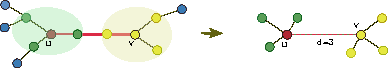
\includegraphics[width=.9\textwidth]{nspdk}
\caption{Pairwise neighborhood subgraphs for the ``red'' node with $r=1$ and $d=3$}
\label{fig:nspdk}
\end{figure}

\subsubsection{Graph node kernels}
The state of the art kernels are based on diffusion phenomenon. In other words, they take paths connecting two nodes into account when measuring their similarity. In the following, we shortly introduce some of the most used graph node kernels.

\begin{itemize}


\item Laplacian exponential diffusion kernel: One of the most well-known graph node kernels is the Laplacian exponential diffusion kernel LEDK, as it is widely used for exploiting discrete structures in general and graphs in particular. On the basis of the heat diffusion dynamics, Kondor and Lafferty proposed LEDK in \cite{kondor2002diffusion}: imagine to initialize each vertex with a given amount of heat and let it flow through the edges until an arbitrary instant of time. The similarity between any vertex couple $v_{i}$, $v_{j}$ is the amount of heat starting from $v_{i}$ and reaching $v_{j}$ within the given time. Therefore, LEDK can capture the long range relationship between vertices of a graph to define the global similarities. Below is the formula to compute LEDK values:
\begin{equation} 
\label{LEDK-formula}
K = e^{-\beta L} = I - \beta L + \frac{\beta L^{2}}{2!} - ...
\end{equation}
where $\beta$ is the diffusion parameter and is used to control the rate of diffusion and $I$ is the identity matrix. Choosing a consistent value for $\beta$ is very important: on the one side, if $\beta$ is too small, the local information cannot be diffused effectively and, on the other side, if it is too large, the local information will be lost. LEDK is positive semi-definite as proved in \cite{kondor2002diffusion}.

\item Exponential diffusion kernel: In LEDK, the similarity values between high degree vertices are generally higher compared to those between low degree ones. Intuitively, the more paths connect two vertices, the more heat can flow between them. This could be problematic since peripheral nodes have unbalanced similarities with respect to central nodes. In order to make the strength of individual vertices comparable, a modified version of LEDK is introduced by Chen et al in \cite{chen2014disease}, called Markov exponential diffusion kernel MEDK and given by the following formula:
\begin{equation} \label{MEDK-formula}
K = e^{-\beta M}
\end{equation}
The difference with respect to the Laplacian diffusion kernel is the replacement of $L$ by the matrix $M=(D-A-nI)/n$ where $n$ is the total number of vertices in graph. The role of $\beta$ is the same as for LEDK.

\item Markov diffusion kernel: The original Markov diffusion kernel MDK was introduced by Fouss et al. \cite{fouss2006experimental} and exploits the idea of diffusion distance, which is a measure of how similar the pattern of heat diffusion is among a pair of initialized nodes. In other words, it expresses how much nodes "influence" each other in a similar fashion. If their diffusion ways are alike, the similarity will be high and, vice versa, it will be low if they diffuse differently. This kernel is computed starting from the transition matrix $P$ and by defining $Z(t) = \frac{1}{t}\sum_{\tau=1}^{t}P^{\tau}$, as follows:
\begin{equation} 
\label{MDK-formula}
K = Z(t)Z^{\top}(t)
\end{equation}

\item Regularized Laplacian kernel: Another popular graph node kernel function used in graph mining is the regularized Laplacian kernel RLK. This kernel function is introduced by Chebotarev and Shamis in \cite{chebotarev2006matrix} and represents a normalized version of the random walk with restart model. It is defined as follows:
\begin{equation} 
\label{RLK-formula}
K = \sum_{n=0}^{\infty}\beta^{n}(-L)^n = (I + \beta L)^{-1}
\end{equation}
where the parameter $\beta$ is again the diffusion parameter. RLK counts the paths connecting two nodes on the graph induced by taking $-L$ as the adjacency matrix, regardless of the path length. Thus, a non-zero value is assigned to any couple of nodes as long as they are connected by any indirect path. RLK remains a relatedness measure even when diffusion factor is large, by virtue of the negative weights assigned to self-loops.

\end{itemize}
\section{Method}
\label{method}
We start from the type of similarity notion computed by a neighborhood based decomposition kernel between graph instances \cite{costa2010fast}, NSPDK, and adapt it to form a convolutional graph node kernel which aims at expressing the similarity between nodes in a single graph. Our intended graph node kernel takes an undirected, labeled graph as its input.

Given an input labeled graph $G=(V,E, \mathcal{L}_1, \mathcal{L}_2)$, our kernel consists of two phases. In the first phase, a network decomposition procedure is applied to transform the graph into a set of linked sparse connected components. In this procedure, we define two different kinds of link: \textit{conjunctive} and \textit{disjunctive} in which we treat them in distinct manners. In the second step, the similarity between any node couple ($u$, $v$) is computed by adopting NSPDK on two neighborhood subgraphs rooted as $u$ and $v$ which extracted from the resulted graph after decomposing. In the following, we describe each phase in detail.

\subsection{Network Decomposition} 
\label{network-decomposition}
In genetic networks, it is not uncommon to find nodes with high degrees. Unfortunately these cases cannot be effectively processed by a neighborhood based decomposition kernel (see \ref{graph-kernels}) since these are based on the notion of exact matches. Neighborhood subgraphs rooted at high degree nodes are relatively big due to a high number of neighbors and edges. It leads to a low likelihood of finding neighborhood subgraphs rooted at high degree nodes which are isomorphic. Thus, the probability of having identical neighborhoods decreases exponentially as the degree increases. This means that in a finite network it quickly becomes impossible to find any match and hence learn or generalize at all. 

We propose a procedure to ``sparsify'' the network that is observed by the neighborhood kernel. In practice, we mostly keep the same the cardinality of the edge set. However we mark the edges with special attributes so that kernel is able to treat them differently when computing. The result is a procedure that decomposes the network in a linked collection of sparse sub-networks where each node has a reduced connectivity when considering the edges of a specific type. However the other edges are still available to connect the various sub-networks. We distinguish two types of edges: {\em conjunctive} and {\em disjunctive} edges. Nodes linked by conjunctive edges are going to be used jointly to define the notion of context and will be visible to the neighborhood graph kernel. Nodes linked by disjunctive edges are instead used to define features based only on the pairwise co-occurrence of the genes at the endpoints and are processed by our novel kernel.

\textit{Iterative k-core decomposition} \cite{alvarez2005k}: the node set is partitioned in two groups on the basis of the degree of each node w.r.t. a threshold degree $D$, the first part contains all nodes with degree smaller than or equal to $D$ and the second part the remaining ones. The node partition is used to induce the ``conjunctive'' vs ``disjunctive'' notion for the edge partition: edges that have both endpoints in the same part are marked as conjunctive, otherwise they are marked as disjunctive. We apply the k-core decomposition iteratively, where at each iteration we consider only the graph induced by the conjunctive edges. We stop iterating the decomposition after a user defined number of steps. Note that this decomposition does not alter the cardinality of the edge set, it is simply a procedure to mark each edge with the attribute conjunctive or disjunctive.  

\begin{figure}
\centering
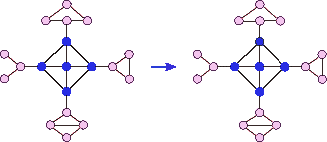
\includegraphics[width=.9\textwidth]{k_core}
\caption{K-core decomposition with degree threshold $D = 4$}
\label{fig:kcore-decomposition}
\end{figure}

\textit{Clique decomposition} \cite{tarjan1985decomposition}: to model the notion that nodes in a clique are tightly related, we summarize the whole clique with a new ``representative'' node. All the cliques (completely connected subgraphs) with a number of nodes greater than or equal to a given threshold size $C$ are identified. The endpoints of all edges incident on the clique's nodes are moved to the representative node. Disjunctive edges are introduced to connect each node in the clique to the representative. Finally all edges with both endpoints in the clique are removed.

In our work a network is transformed by applying first the iterative k-core decomposition and then the clique decomposition.

\begin{figure}
\centering
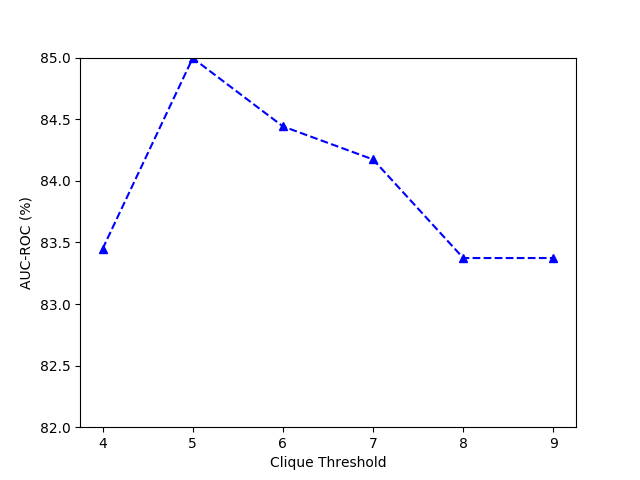
\includegraphics[width=.9\textwidth]{cliques}
\caption{Clique decomposition with threshold $C = 4$}
\label{fig:clique-decomposition}
\end{figure}

\subsection{The Conjunctive Disjunctive Node Kernel}
%We start from the Neighborhood Subgraph Pairwise Distance Kernel (NSPDK) \cite{costa2010fast} and adapt it to express the similarity between nodes in a single network. The key idea in NSPDK is to decompose graphs in small fragments and count how many pairs of fragments are shared between two instances. We introduce two improvements: \textit{i}) we partition the features according to the individual node's neighborhood, and \textit{ii}) we introduce a  distinction between ``disjunctive'' and ``conjunctive'' edges.

We define a node kernel $K(G_u,G_{u'})$ between two copies of the same network $G$ where we distinguish the nodes $u$ and $u'$ respectively. The idea is to define the features of a node $u$ as the subset of NSPDK features that always have the node $u$ as one of the roots. In addition we distinguish between two types of edges, called {\em conjunctive} and {\em disjunctive} edges. When computing distances to induce neighborhood subgraphs, only conjunctive edges are considered. When choosing the
pair of neighborhoods to form a single feature, we additionally consider roots $u$ and $v$ that are not at distance $d$ but such that $u$ is connected to $w$ via a disjunctive edge and such that $w$ is at distance $d$ from $v$ (Figure \ref{fig:cdnk} is an illustration). In this way disjunctive edges can still allow an {\em information flow} even if their
endpoints are only considered in a pairwise fashion and not jointly. 

Formally, we define two relations: the \textit{conjunctive relation} $R^{\wedge}_{r,d}(A_u, B_v, G_u)$ identical to the NSPDK relation $R_{r,d}(A_u, B_v, G)$,  and (ii) $\mathcal{D}(u,v)= d$; the \textit{disjunctive relation} $R_{r,d}^{\vee}(A_u, B_v, G_u)$ is true {\em iff} (i)  $A_u \cong \mathcal{N}_r^u$ and $B_v \cong \mathcal{N}_r^v$ are true, (ii) $\exists w$ s.t. $\mathcal{D}(w,v)= d$, and (iii) $(u,w)$ is a disjunctive edge. We define $\kappa_{r,d}$ on the  inverse relations ${R^{\wedge}_{r,d}}^{ -1}$ and ${R^{\vee}_{r,d}}^{ -1}$:
\begin{center}
 $\kappa_{r,d}(G_u,G_{u'}) = \!\!\!\!\!\!\!\!\!\!\!\!
 \sum\limits_{\substack {A_u,{B}_{v} \in {R_{r,d}^{\wedge}}^{ -1}(G_u) \\ A'_{u'},{B'}_{v'} \in {R_{r,d}^{\wedge}}^{ -1}(G_{u'}) }} \!\!\!\!\!\!\!\!\!\!\!\!
  { \textbf{1}_{A_u \cong A'_{u'}} \cdot { \textbf{1}_{B_{v} \cong B'_{v'}}}}
+ \!\!\!\!\!\!\!\!\!\!\!\!
 \sum\limits_{\substack {A_u,{B}_{v} \in {R_{r,d}^{\vee}}^{ -1}(G_u) \\
  A'_{u'},{B'}_{v'} \in \ {R_{r,d}^{\vee}}^{ -1}(G_{u'}) }} \!\!\!\!\!\!\!\!\!\!\!\!
  { \textbf{1}_{A_u \cong A'_{u'}} \cdot { \textbf{1}_{B_{v} \cong B'_{v'}}}}
  $.
\end{center}
The CDNK is finally defined as $K(G_u,G_{u'}) = \sum\limits_{r}{\sum\limits_{d}{\kappa_{r,d}(G_u,G_{u'})}}$, where once again for efficiency reasons, the values of $r$ and $d$ are upper bounded to a given maximal $r^*$ and $d^*$.

\begin{figure}
\centering
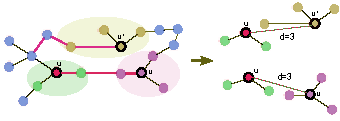
\includegraphics[width=.9\textwidth]{cdnk}
\caption{Pairwise neighborhood subgraphs for the ``red'' node with $r=1$ and $d=3$ using ``\textit{conjuction}'' and ``\textit{disjuctive}'' edges}
\label{fig:cdnk}
\end{figure}

In order to integrate the information of real vector labels, we proceed as follows. We compute a sparse vector representation for the neighborhood graph rooted in node $v$ following \cite{costa2010fast}: for each neighborhood subgraph we calculate the quasi-isomorphism certificate hash code; we then combine the hashes for the pair of neighborhoods and use the resulting integer as a feature indicator. This yields a direct sparse vector representation (associated to node $u$ in graph $G$) $f: G_u \longmapsto I\!R^N$ where $N \approx 10K-1M$. Given the real valued vector information (associated to node $u$ in graph $G$) $g: G_u \longmapsto I\!R^P$ computed as the multi-class similarity to the $P$ clusters (c.f.r. Section \ref{sec:lab}), we update the computation of CDNK considering the discrete convolution of the discrete information with the real valued information:   
\begin{equation}
K(G_u,G_{u'}) = \left< f(G_u) \bigotimes g(G_u), f(G_{u'}) \bigotimes g(G_{u'}) \right>,
\end{equation}
where the discrete convolution is defined as: 
$(f \bigotimes g)[n]=\sum _{m=0}^{K-1}f[n-m]g[m].$
In words, we are starting a scaled copy of the real valued vector at the position indicated by each feature computed on the basis of the discrete information. Intuitively, when both the real valued and the discrete information match, the kernel computes a large similarity, but if there is a discrepancy in either one of the sources of information, the similarity will be penalized. 

\section{Parameter Space}
Our kernel consists of five parameters: the threshold degree $D$, clique size threshold $C$, maximal radius $r^*$, maximal distance $d^*$ and number of clusters $P$ clusters in which their values are in $\mathbb{N}^*$. In order to choose the optimal tuple of parameters for kernel in a specific setting, a model selection procedure is normally adopted from a determined subset of parameter space. The parameter space of our kernel seems large due to the relatively high number of parameters. However, most parameter values are supposed to be in limited ranges. Therefore, it is actually not too big. In particular, the clique size threshold $C$ is recommended to be in $\lbrace 4, 5\rbrace$. The maximal radius $r^*$ is set with a value smaller than or equal to $3$ since it will lead to big neighborhood subgraphs (as discussed in \ref{network-decomposition}). The maximal distance $d^*$ is assigned with values less than or equal to $4$ because the value of the maximal shortest distance between nodes in a connected component is often not too high. The values of the threshold degree $D$ should neither be too high and too low. If it is high, we have to face with high degree node problem, and if it is too low, the obtained graph consists of too sparse connected components. Therefore, we suggest the value for $D$ is in $\left[6, 20 \right]$. 

\section{Empirical Evaluation}
\label{empirical-evaluation-cdnk}
In this section, we desire to evaluate the performance of CDNK and other graph node kernels to answer for the two following questions:
\begin{itemize}
\item Does CDNK show better performance comparing to other graph node kernels?
\item Does the use of side information (real vector labels) help to improve the performance of CDNK?
\end{itemize}

\subsection{Experimental Settings and Evalution Method}
We carry out experiments in the context of disease gene prioritization where the aim is to build a learning system which allows to prioritize candidate genes based on their probabilities of being associated to a given genetic disease.

 Given a genetic graph and a list of training genes known to cause a genetic disease. We first apply  a graph node kernel to compute kernel matrix. This kernel matrix together with training gene set are used as the input of a learning algorithm to construct a model. The obtained model is then used to prioritize for candidate genes.

The experiments are performed on two separate networks derived from BioGPS and Pathways datasets in which we follow the experiment procedure in \cite{chen2014disease} where 12 diseases \cite{goh2007human} are used in which each disease is associated to at least 30 positive genes (see table \ref{tab:cdnk-diseases} for the list of genetic diseases and the number of positive genes in each disease). For each disease, we construct a positive set $\mathcal{P}$ with all positive (confirmed) disease genes, and a negative set $\mathcal{N}$ which contains random genes associated at least to one disease class which is not related to the class that is defining the positive set. In \cite{chen2014disease} the ratio between the dataset sizes is chosen as $\vert \mathcal{N} \vert = \frac{1}{2} \vert \mathcal{P} \vert$. This is due to the fact that genes known to be related to at least a genetic disease, but not to the considered one are well studied, so they have low probability to be associated to the current disease.
\begin{itemize}
\item \textbf{BioGPS:} A gene co-expression network is constructed from BioGPS dataset, which contains 79 tissues, measured with the Affymetrix U133A array. Edges are inserted when the pairwise Pearson correlation coefficient (PCC) between genes is larger than 0.5.

\item \textbf{Pathways:} Pathway information is retrieved from KEGG, Reactome, PharmGKB and the Pathway Interaction Database. If a couple of proteins co-participate in any pathway, the two corresponding genes are linked.  
\end{itemize}
To compare the performance of graph node kernels, we fix the learning algorithm and sequentially substitute differnt graph node kernels. The performance of the system obtained in different cases are used to compare the performance of the employed graph node kernels: LEDK, MEDK, MDK, RLK and CDNK.

The predictive performance of the system using each kernel is evaluated via a leave-one-out cross validation: one gene is kept out in turn and the rest are used to train an SVM model. We compute a decision score $q_i$ for the test gene $g_i$ as the top percentage value of score $s_i$ among all candidate gene scores. We collect all decision scores for every gene in the test set to form a global decision score list on which we compute the AUC-ROC.

\subsection{Node Labeling} 
\label{sec:lab}
The graph node kernel takes the labled graphs as its input in which labels can be discrete and/or real valued vectors. Therefore, to carry out experiments on graphs derived from BioGPS and Pathways, we need ways to label for these genetic graphs. Following are our proposed node labeling methods for genetic networks. Note that we allow the user to define and use any node labeling functions which are informative.

\textit{Discrete labels:} We cast two different approaches to associate genes with dicrete labels.

The first approach, we use a same label for every node of graphs. In this case, the configuration of nodes expressed by the pairwise neighborhood subgraphs in CDNK now turn to pairwise neighborhoods. Besides, since labels are identical, the cardinality of neighborhoods are took into account.

The second approach aims to use nodes labels to encode abstract information about the genes. In this way downstream machine learning algorithms can generalize from similar examples and allow the identification of overlooked but related genes. We employ a gene ontology \cite{gene2004gene} to construct binary vectors representing a bag-of-words encoding for each gene, i.e. each element of a binary vector is equal to 1 if its corresponding GO-term is associated to the gene, and is equal to 0 otherwise.). The resulting vectors are then clustered using the k-means algorithm into a user defined number of classes, $P$, so that genes with similar description profiles receive the same class identifier as label.

\textit{Real vector labels:} In addition to encoding the functional information as a discrete label we add a richer description by computing the similarity vector w.r.t. to each cluster. In this way we can fully exploit the latent description of the genes in terms of the different functional groups captured by the clustering procedure. Formally, given a vector $v \in I\!R^{26501}$ we compute a similarity vector $S(v)= {s_1, s_2, \ldots s_P}$ with entries $s_i = \frac{1}{1+ \ell(v,c_i)}$ where $\ell(v,c_i)$ is the Euclidean distance of $v$ from the center of the $i^{th}$ cluster $c_i = \frac{1}{|C_i|}\sum_{x \in C_i} x$ computed as the geometric mean of the elements in the cluster $C_i$.

\subsection{Model Selection}
The hyper parameters of the various methods are tuned using a k-fold cross validation. However due to the non i.i.d. nature of the problem, we employ a stronger setup to ensure no information leakage. The dataset on which we are validating the performance is never subsequently used in the predictive performance estimation. The values for diffusion parameter $\beta$ in LEDK and MEDK are sampled in $\lbrace 10^{-3}, 10^{-3}, 10^{-2}, 10^{-1} \rbrace$, time steps $t$ in MDK in $\lbrace 1, 10, 100 \rbrace$ and RLK parameter $\beta$ in $\lbrace 1, 4, 7 \rbrace$. For CDNK, the degree threshold values, $D$, are sampled in $\lbrace 10,\ 15,\ 20 \rbrace$, clique size threshold, $C$, in $\lbrace 4,\ 5 \rbrace$, maximum radius, $r^*$, in $\lbrace 1,\ 2 \rbrace$, maximum distance, $d^*$, in $\lbrace 2,\ 3,\ 4 \rbrace$, number of clusters $P$ in $\lbrace 5,\ 7 \rbrace$. Finally, the regularization trade off parameter $C$ for the SVM is sampled in $\lbrace 10^{-5},  \ 10^{-4}, \ 10^{-3},\ 10^{-2},\ 10^{-1}, 1,\ 10,\ 10^2 \rbrace$.

\subsection{Parameter Impact}
In order to evaluate the stability of kernel w.r.t the change of each parameter values, we perform experiments with disease-gene association 2 and on the BioGPS network. For each parameter, first fix the values of all other parameters, but allow the value of this papameter to change. More precisely, we use the optimal tuple $C = 5, d^* = 1, D = 20, P = 15$ for the fixed of parameters' values. We let the changes of $C$ in $\lbrace 4, 5, 6, 7, 8, 9\rbrace$, $d^*$ in $\lbrace 1, 2, 3, 4\rbrace$, $D$ in $\lbrace 8, 10,  15, 20, 30, 40, 50\rbrace$ and real vector size, $P$ in $\lbrace 8, 10,  15, 20, 30, 50, 70, 90\rbrace$

\subsection{Results and Discussion}
Table \ref{fig:cdnk-biogps} and \ref{fig:cdnk-pathways} show the AUC-ROC performance of different models using state of the art graph node kernels and different variations of CDNK on BioGPS and Pathways networks, respectively. In what follows, we analyze the results to answer for the two questions which are previously raised.

Concering the performance of different graph node kernels, CDNK variations outperform diffusion-based graph node kernels in all cases on BioGPS dataset and 8 out of 11 cases on Pathways when compared to diffusion-based kernels. CDNK is ranked first when considering both the average AUC-ROC and the average rank with a difference, w.r.t. the best diffusion-based kernel, ranging from 5.4$\%$ to 10$\%$ and from 1.2$\%$ to 3.4$\%$ on BioGPS and Pathways, respectively. As a consequence, we can conclude that CDNK show state of the art performance in graph node kernels.

Regarding the variations of CDNK, the integration of real valued vectors improves the performance in most cases. In particular, considering the use of discrete labels based on ontology, using side information helps to increase the performance in all diseases on BioGPS and in 9 out of 11 diseases on Pathways. Similarly, by employing auxiliary information associated to graph nodes, the performance of CNDK in case of using uniform discrete labels is also improved in 9 and 8 out of 11 on BioGPS and Pathways, respectively.
%==================================================
\section{Conclusion and Future Work}
We have shown how decomposing a network in a set of connected sparse graphs allows us to take advantage of the discriminative power of CDNK, a novel decomposition kernel, to achieve state-of-the-art results. Moreover, we have also introduced the way to integrate ``side'' information in form of real valued vectors when it is available on graph to get even better performance of CDNK. In future work we will investigate how to \textit{i}) decompose networks in a data driven way and \textit{ii}) extend the CDNK approach to gene-disease association problems exploiting multiple heterogeneous information sources in a joint way.
%======================================================
%==================================================
%==================================================
\begin{table}
\caption{\textit {Predictive performance on 11 gene-disease associations in percentage using network induced by the BioGPS. Best results in bold. We report the AUC ROC and the rank for each kernel method.  CDNK1 = ontology for discrete labels, CDNK2 = ontology for both discrete and vector labels, CDNK3 = uniform discrete labels and CDNK4 = uniform discrete labels and ontology for vector label.}} \vspace{1em}
%\vspace*{5pt}
\centering
\setlength{\tabcolsep}{1mm}
\begin{tabular}{|c|c|c|c|c|c|c|c|c|}
\hline
         & \multicolumn{8}{c|}{\textbf{BioGPS}}\\
 \hline
Disease & DK & MD & MED & RL & CDNK1 & CDNK2 & CDNK3 & CDNK4\\

 \hline
1 & 51.9/8 & 57.4/7 & 59.0/6 & 59.2/5 & 65.1/4 & 69.5/3 & 72.0/2 & \textbf{72.3/1} \\

2 & 81.7/5 & 78.5/6 & 75.2/7 & 75.0/8 & 88.3/2 & \textbf{88.8/1} & 83.2/4 & 84.8/3 \\

3 & 64.3/6 & 59.6/8 & 71.6/3 & 71.8/2 & 65.5/5 & \textbf{72.5/1} & 61.4/7 & 67.9/4 \\

4 & 65.3/7 & 58.2/8 & 67.8/6 & 67.8/5 & 71.9/4 & \textbf{78.7/1} & 73.8/3 & 76.7/2 \\

5 & 64.0/8 & 64.1/7 & 66.5/5 & 66.2/6 & 75.9/4 & 76.2/3 & 77.8/2 & \textbf{78.2/1} \\

6 & 74.6/5 & 70.2/8 & 71.0/7 & 71.2/6 & 79.3/3 & \textbf{83.7/1} & 77.2/4 & 80.0/2 \\

7 & 73.0/5 & 66.7/7 & 75.4/3 & 75.6/2 & 68.8/6 & 73.9/4 & 66.1/8 & \textbf{77.4/1} \\

8 & 74.4/8 & 76.8/3 & 76.2/5 & 76.4/4 & 74.7/7 & 77.7/1 & 76.1/6 & 76.9/2 \\

9 & 71.5/2 & 65.6/8 & 67.7/6 & 69.9/3 & 66.8/7 & \textbf{71.7/1} & 67.9/5 & 68.1/4 \\

10 & 54.0/6 & 50.3/8 & 56.1/5 & 51.1/7 & 77.6/4 & \textbf{82.7/1} & 77.7/3 & 78.3/2 \\

11 & 58.2/7 & 51.3/8 & 59.3/6 & 59.3/5 & 71.8/4 & \textbf{80.2/1} & 74.8/2 & 74.0/3 \\

\hline
$\overline{AUC}$ & 66.6	& 63.5 & 67.8 &	67.6 & 73.2 & \textbf{77.8} & 73.5 & 75.9 \\


$\overline{Rank}$ & 6.09 & 7.09 &  5.36 & 4.82 & 4.45 & \textbf{1.64} & 4.18 & 2.27 \\
 \hline 
\end{tabular}
\label{fig:cdnk-biogps}
\end{table}

%=====================================
%=====================================
\begin{table}
\caption{\textit {Predictive performance on 11 gene-disease associations in percentage using network induced by the Pathways. Best results in bold. We report the AUC ROC and the rank for each kernel method.  CDNK1 = ontology for discrete labels, CDNK2 = ontology for both discrete and vector labels, CDNK3 = uniform discrete labels and CDNK4 = uniform discrete labels and ontology for vector label.}} \vspace{1em}
%\vspace*{5pt}
\centering
\setlength{\tabcolsep}{1mm}
\begin{tabular}{|c|c|c|c|c|c|c|c|c|}
\hline
         & \multicolumn{8}{c|}{\textbf{Pathways}} \\
 \hline
Disease & DK & MD & MED & RL & CDNK1 & CDNK2 & CDNK3 & CDNK4 \\

 \hline
1 & 74.7/8 & 76.4/7 & 78.7/6 & 78.8/5 & 80.2/4 & 82.4/2 & \textbf{82.8/1} & 82.3/3 \\

2 & 55.1/8 & 64.9/7 & 76.6/6 & 76.6/5 & 81.1/2 & 80.3/4 & 80.1/3 & \textbf{81.9/1} \\

3 & 55.0/8 & 62.7/7 & 64.1/5 & 65.6/4 & 67.1/3 & 63.6/6 & 69.7/2 & \textbf{71.4/1} \\

4 & 54.3/8 & 65.2/6 & \textbf{73.7/1} & 73.7/2 & 66.1/5 & 68.1/3 & 64.0/7 & 67.3/4 \\

5 & 52.9/8 & 55.7/7 & 62.7/5 & 62.7/6 & 68.3/2 & \textbf{69.6/1} & 66.2/4 & 68.1/3 \\

6 & 83.4/8 & 92.7/7 & 96.5/2 & \textbf{96.5/1} & 93.0/6 & 94.1/5 & 94.5/4 & 94.9/3 \\

7 & 84.5/7 & 88.3/8 & 89.4/2 & \textbf{89.5/1} & 88.5/6 & 88.5/5 & 89.0/3 & 88.7/4 \\

8 & 53.7/8 & 65.6/7 & 72.0/6 & 72.3/5 & 72.5/4 & 72.5/3 & 74.9/2 & \textbf{75.3/1} \\

9 & 52.5/8 & 64.9/5 & 64.2/7 & 64.2/6 & \textbf{81.3/1} & 81.0/3 & 80.1/2 & 79.8/4 \\

10 & 68.8/6 & 65.4/8 & 74.4/5 & 74.4/4 & 66.9/7 & 76.8/2 & 75.2/3 & \textbf{78.7/1} \\

11 & 53.7/8 & 69.2/7 & 74.6/5 & 74.1/6 & 77.0/3 & \textbf{78.7/1} & 75.1/4 & 77.3/2 \\

\hline
$\overline{AUC}$ & 62.6	& 70.1 & 75.2 & 75.3 & 76.5 & 77.8 & 77.4 &	\textbf{78.7}
 \\
$\overline{Rank}$ & 7.73 & 6.82 & 4.55 & 4.09 & 3.91 & \textbf{2.27} & 3.18 & 2.45 \\
 \hline 
\end{tabular}
\label{fig:cdnk-pathways}
\end{table}

\newpage
\begin{figure}[!tbp]
  \centering
  \begin{minipage}[b]{0.47\textwidth}
    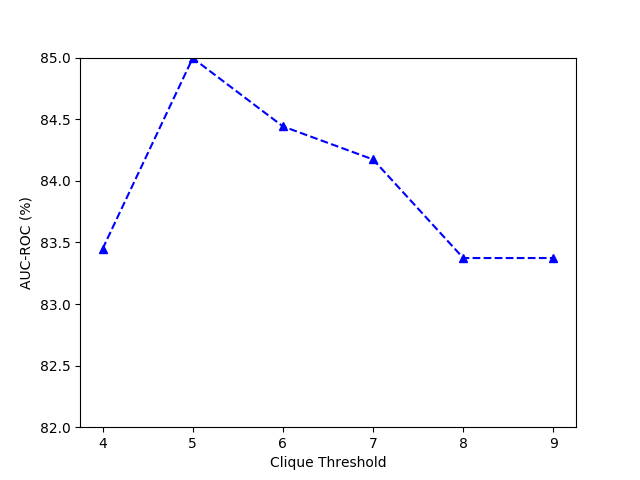
\includegraphics[width=\textwidth]{cliques.png}
    \caption{Performance with C changes}
    \label{fig:c-change}
  \end{minipage}
  \hfill
  \begin{minipage}[b]{0.47\textwidth}
    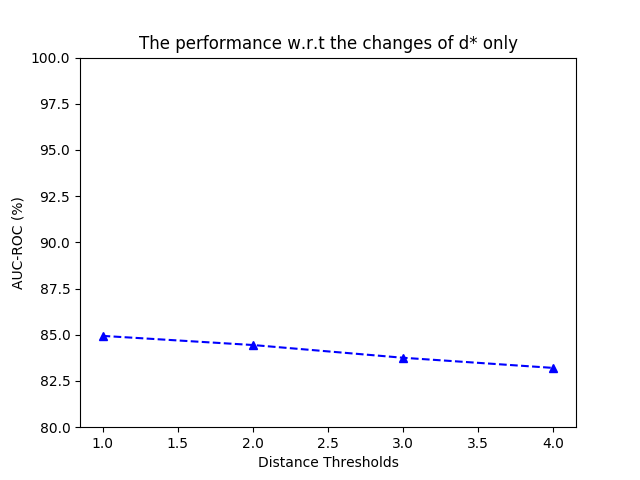
\includegraphics[width=\textwidth]{distance.png}
    \caption{Performance with d* changes}
    \label{fig:d-change}
  \end{minipage}
\end{figure}

\begin{figure}[!tbp]
\centering
  \begin{minipage}[b]{0.47\textwidth}
    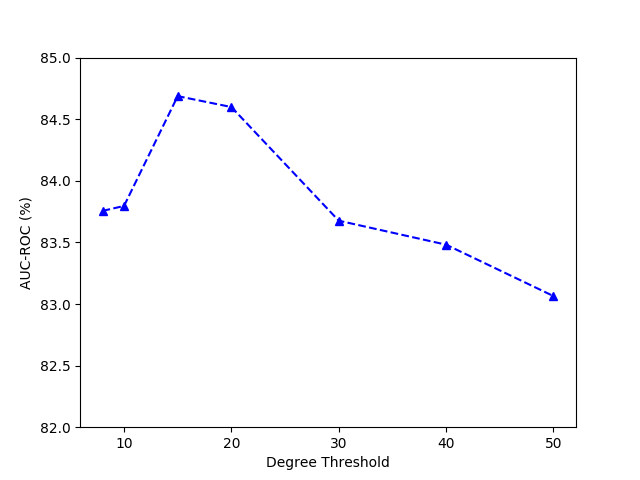
\includegraphics[width=\textwidth]{degree.png}
    \label{fig:D-change}
    \caption{Performance with D changes}
  \end{minipage}
  \begin{minipage}[b]{0.47\textwidth}
    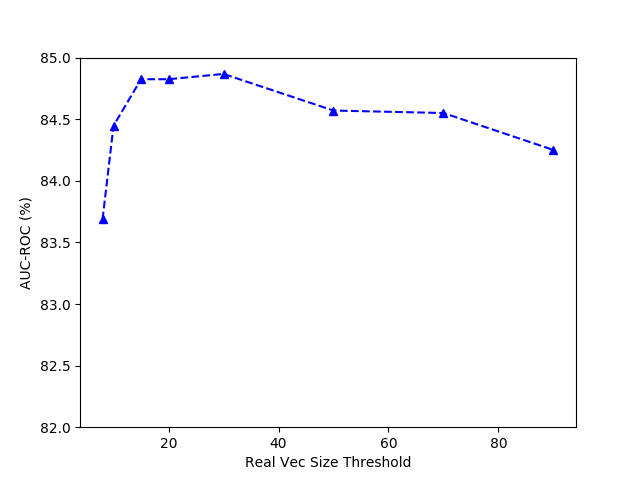
\includegraphics[width=\textwidth]{vec_size.png}
    \label{fig:vs-change}
    \caption{Performance with P changes}
  \end{minipage}  
\end{figure}



\section{Conclusions}
We have shown how decomposing a network in a set of connected sparse graphs allows us to take advantage of the discriminative power of CDNK, a novel decomposition kernel, to achieve state-of-the-art results. Moreover, we have also introduced the way to integrate ``side'' information in form of real valued vectors when it is available on graph to get even better performance of CDNK. In future work we will investigate how to \textit{i}) decompose networks in a data driven way and \textit{ii}) extend the CDNK approach to gene-disease association problems exploiting multiple heterogeneous information sources in a joint way.
%\section{The Elsevier article class}
%
%\paragraph{Installation} If the document class \emph{elsarticle} is not available on your computer, you can download and install the system package \emph{texlive-publishers} (Linux) or install the \LaTeX\ package \emph{elsarticle} using the package manager of your \TeX\ installation, which is typically \TeX\ Live or Mik\TeX.
%
%\paragraph{Usage} Once the package is properly installed, you can use the document class \emph{elsarticle} to create a manuscript. Please make sure that your manuscript follows the guidelines in the Guide for Authors of the relevant journal. It is not necessary to typeset your manuscript in exactly the same way as an article, unless you are submitting to a camera-ready copy (CRC) journal.
%
%\paragraph{Functionality} The Elsevier article class is based on the standard article class and supports almost all of the functionality of that class. In addition, it features commands and options to format the
%\begin{itemize}
%\item document style
%\item baselineskip
%\item front matter
%\item keywords and MSC codes
%\item theorems, definitions and proofs
%\item lables of enumerations
%\item citation style and labeling.
%\end{itemize}
%
%\section{Front matter}
%
%The author names and affiliations could be formatted in two ways:
%\begin{enumerate}[(1)]
%\item Group the authors per affiliation.
%\item Use footnotes to indicate the affiliations.
%\end{enumerate}
%See the front matter of this document for examples. You are recommended to conform your choice to the journal you are submitting to.
%
%\section{Bibliography styles}
%
%There are various bibliography styles available. You can select the style of your choice in the preamble of this document. These styles are Elsevier styles based on standard styles like Harvard and Vancouver. Please use Bib\TeX\ to generate your bibliography and include DOIs whenever available.
%
%Here are two sample references: \cite{Feynman1963118,Dirac1953888}.
\section*{Funding}
This work was supported by the University of Padova, Strategic Project BIOINFOGEN.
\section*{References}

\bibliography{mybibfile}

\end{document}
